%!TEX root = ../report.tex
%*******************************************************************************
%                               State of The Art                               %
%*******************************************************************************


\chapter{State of The Art}


\section{Introduction}
    Before elaborating our solution, we discuss in this section some existing approaches and their
    limitations. We define, after, multiple technologies and concepts we use in this project.

\section{Critical overview of the existing}
    There has not been other trials that use the same approach as this project, but there are some other
    attempts to remedy the problem of energy consumption in the IT field. Those solution suggest that
    datacenters should be powered using renewable energy sources.

    \subsection{Solar-Powered Data Centers}
        Emerson Network Power, i/o Data Centers and AISO are among the companies that have implemented on-site
        solar solutions. Emerson Network Power has installed a 7,800 square foot solar array on the roof of its
        new St. Louis data center\cite{emerson-network-power-data-centers}.

        \begin{figure}[!h]\centering
            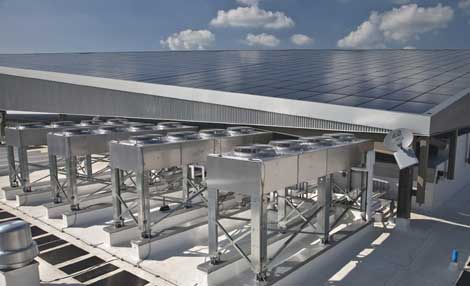
\includegraphics[width=.4\columnwidth]{3-State-of-the-art/figs/emerson-solar-panels.jpg}
            \caption{Emerson Network Power solar array}
        \end{figure}

        Also, QTS Princeton data center campus installed more than 57,000 solar panels in New Jersey countryside.
        The installation generates up to 14.1 megawatts of power. That's more than enough to supply the daytime
        energy needs of the data center\cite{qts-princeton-data-centers}.

        \begin{figure}[!h]\centering
            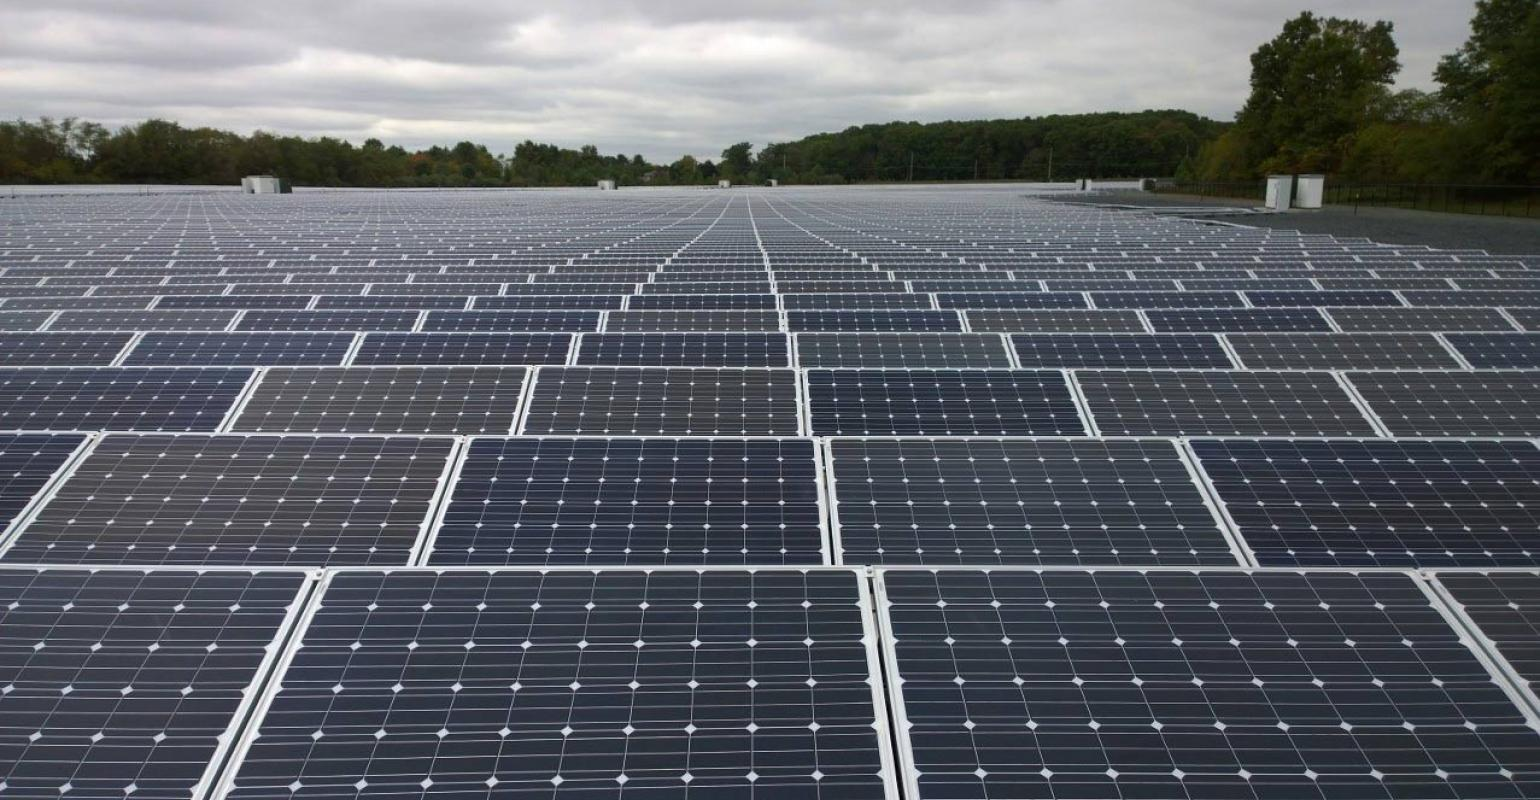
\includegraphics[width=.4\columnwidth]{3-State-of-the-art/figs/qts-solar-panels.jpg}
            \caption{QTS Princeton datacenter photovoltaic solar panels}
        \end{figure}

    \subsection{Wind-Powered Data Centers}
        Only a handful of companies have implemented wind turbines in working data centers.
        A small ISP and hosting company in Woodstock, Illinois, Other World Computing (OWC) may be the first
        data center operator in the U.S. to power its facility entirely with wind power from an on-site turbine.
        In 2009, OWC began using a 131-foot-tall wind turbine to provide all the electric power for its
        building, which includes the company’s headquarters and a data center supporting its web hosting and
        ISP services\cite{wind-powered-data-centers}.

        \begin{figure}[!h]\centering
            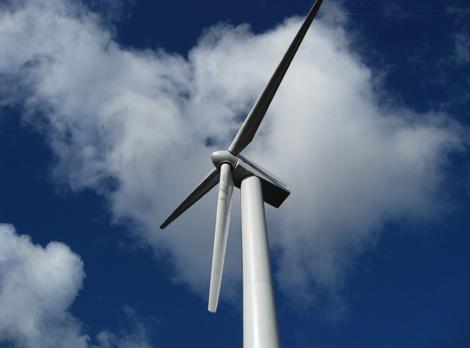
\includegraphics[width=.4\columnwidth]{3-State-of-the-art/figs/owc-wind-turbine.jpg}
            \caption{The 131-foot tall wind turbine at Other World Computing in Woodstock, Illinois}
        \end{figure}

    \subsection{Geothermal Data Centers}
        A number of big companies like Google and Facebook are using geothermal cooling in their data centers.
        They have built them in icy areas like Sweden and Finland taking advantage of the cold air in those
        regions.

    \subsection{Limitations of previous solutions}
        Even though most of these approaches exist in real world, they still have problems reaching the scale
        required to successfully support the power requirements of big data centers.
        Solar power hasn’t been widely used in data centers because it takes a very large installation of
        photovoltaic (PV) solar panels to produce even a fraction of the energy required by most data centers.
        In addition to that, the cost of deploying such solutions is still exorbitant.

        Furthermore, working on the datacenter itself does not take advantage of the vast network of connected
        devices all over the world and keeps these important resources idle and not effectively used.


\section{State of the art}
    In this section, we explain some key concepts and technologies we used during this project. Some of them
    are distributed systems related and some others describe some blockchain notion.
    \begin{itemize}
        \item \textbf{Ethereum blockchain:}

        \begin{figure}[!h]\centering
            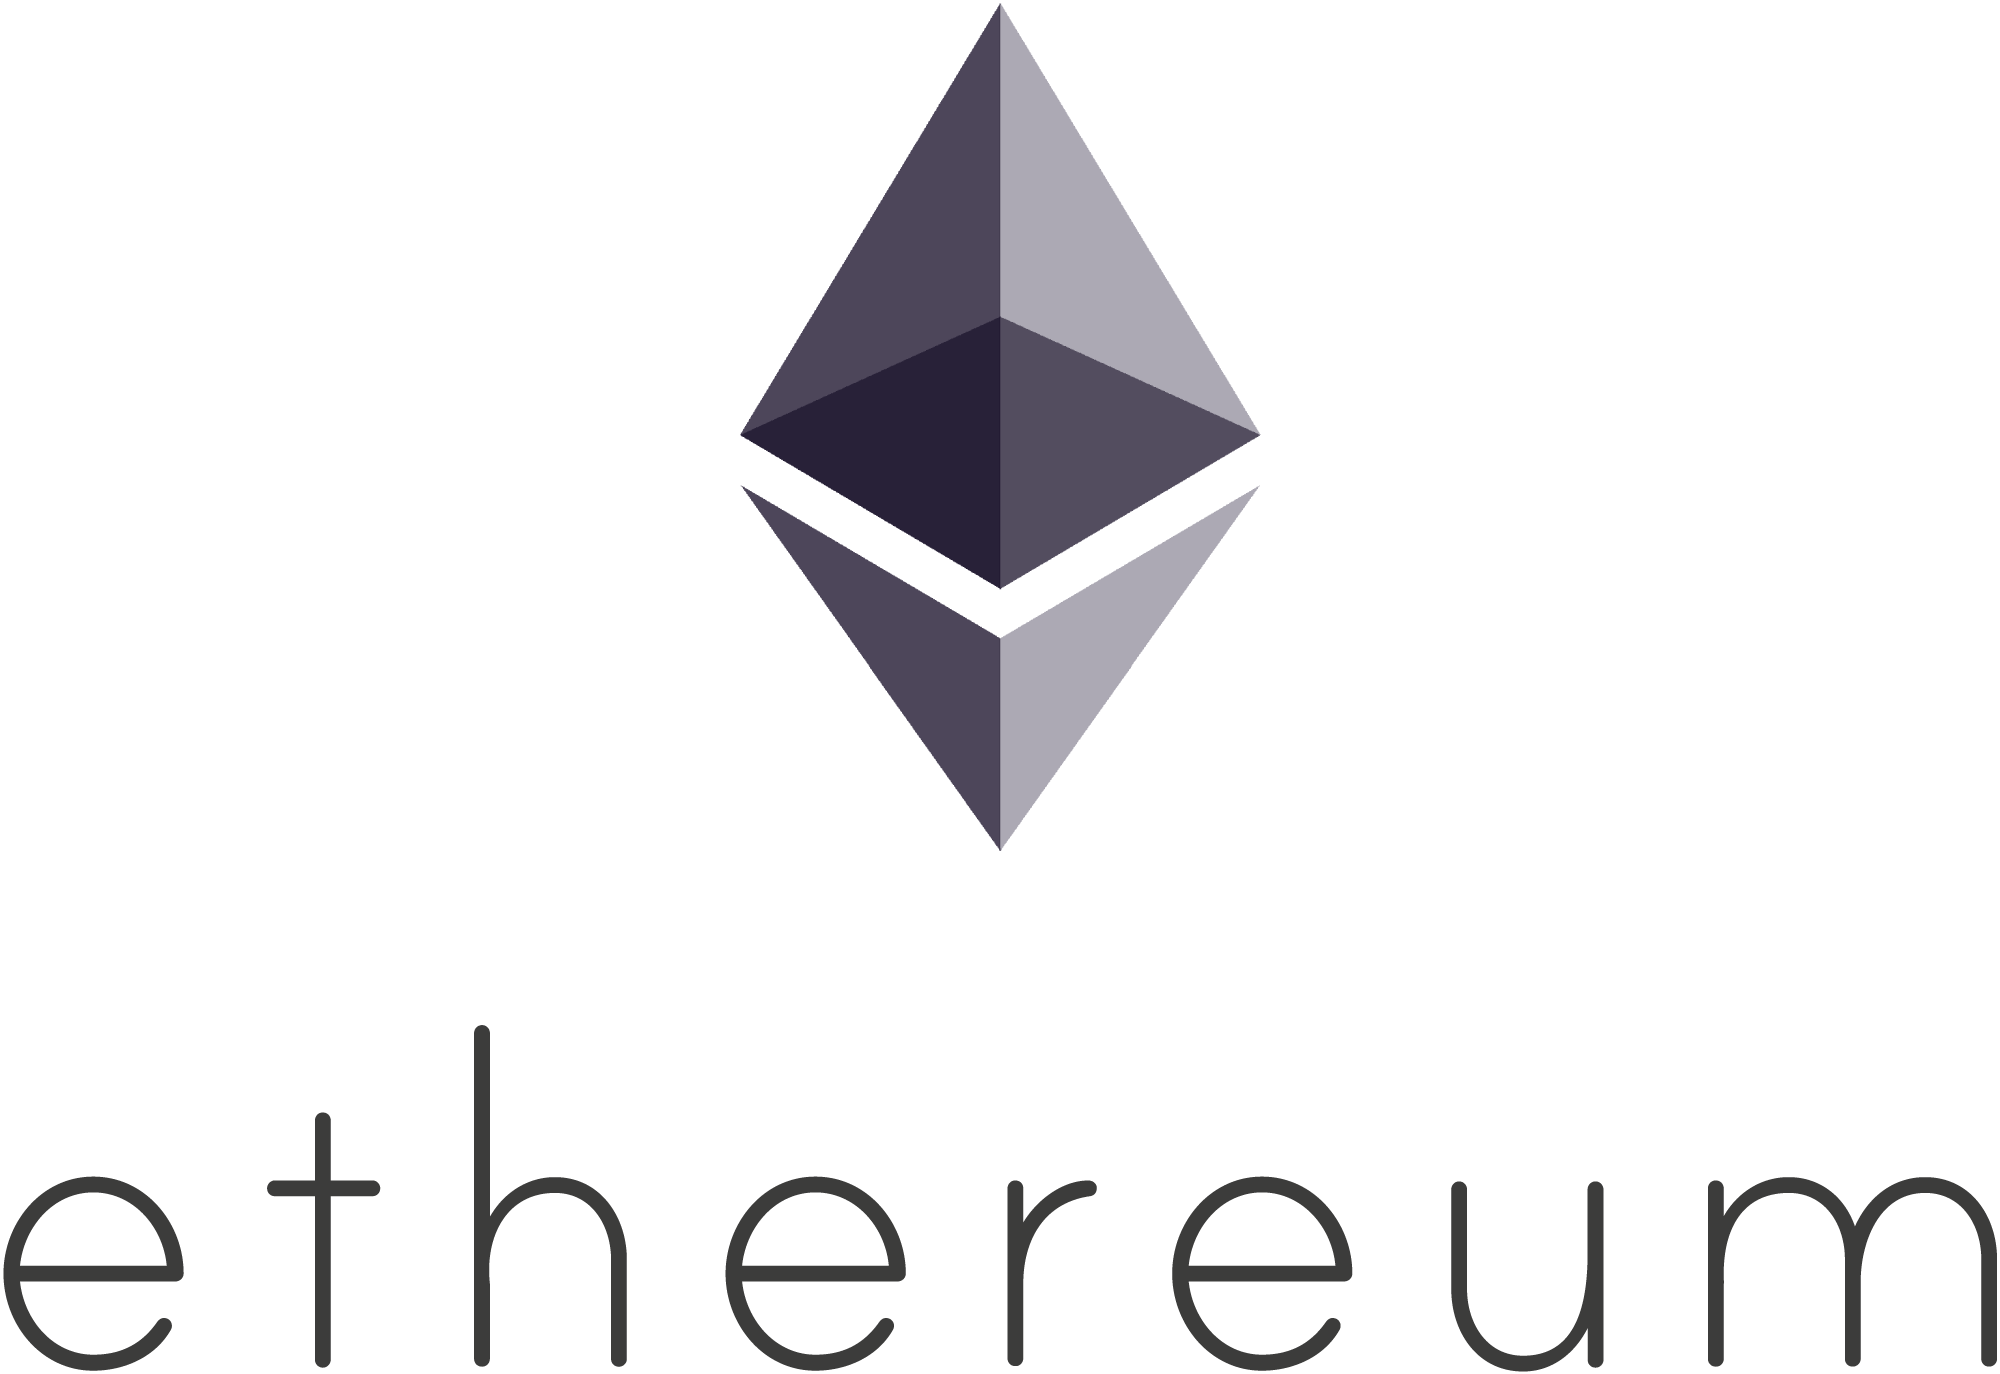
\includegraphics[width=.3\columnwidth]{3-State-of-the-art/figs/ethereum.png}
            \caption{Ethereum blockchain}
        \end{figure}
        
        Ethereum\cite{ethereum} was initially described by Vitalik Buterin\cite{v-buterin} in late 2013
        as a result of his research and work in the Bitcoin community. Vitalik published the Ethereum
        white paper, where he describes in detail the technical design and rationale for the Ethereum
        protocol and smart contracts architecture. In January 2014, Ethereum was formally announced by
        Vitalik at the The North American Bitcoin Conference in Miami, Florida, USA.

        It is an open Blockchain platform that lets anyone build and use decentralized
        applications. Like Bitcoin, no one controls or owns Ethereum – it is an open-source project built
        by the community around the world. But unlike the Bitcoin protocol, Ethereum was designed to be
        adaptable and flexible. It is easy to create new applications on the Ethereum platform.
        
        Ethereum is a programmable Blockchain. Rather than giving users a set of pre-defined operations
        (e.g. Bitcoin transactions), Ethereum allows users to create their own operations of any complexity
        they wish. In this way, it serves as a platform for many different types of decentralized applications,
        including but not limited to cryptocurrencies.
        
        So basically, ethereum allows exchanging ether which makes it behave like Bitcoin does. However,
        ethereum allows anybody to write any piece of code (Smart Contract) and upload it to the Blockchain
        so anyone can interct with it which brings us to cite that there is two types of accounts that lives
        within the ethereum Blockchain: externally owned accounts which are controlled by private keys and
        contrat accounts which are controlled by a piece of code.
        
        It is the Ethereum Virtual Machine (EVM) that executes the code of smart contracts and it is
        generally expensive to run applications on top of ethereum because of gaz price, so iExec's
        plateform takes this execution offchain in order to allow on-demand, secure and low-cost access to
        competitive computing infrastructures.

        \item \textbf{XtremWeb\cite{xtremweb}:} a data driven volunteer cloud middleware used by iExec to manage
        the offchain computations. The middleware implements many features needed such as authentication,
        tasks scheduling, fault-tolerance, security (...). \newline
        It was mainly developed by Oleg Lodygensky\cite{oleg-lodygensky} at the LAL laboratory in IN2P3 based on
        XtremWeb 1.8.0 by INRIA.

        \item \textbf{RLC\cite{RLC}:}

        \begin{figure}[!h]\centering
            
\includegraphics[width=.3\columnwidth]{3-State-of-the-art/figs/RLC.png}
            \caption{RLC token}
        \end{figure}

        It is the token used to access the resources provided by the market network.
        It is the unique way of payment for application providers, server providers and data providers.

        \item \textbf{iExec Software Development Kit\cite{iexec-sdk} (SDK):} this tool gives the ability to
        deploy any legacy applications in the iExec infrastructure, and execute them through calls to
        Ethereum smart contracts.

        \item \textbf{PoCo:} the Proof-of-Contribution protocol\cite{POCO} ensures that the results computed by the
        workers are valid and can be trusted by the user who required them. It controls the way multiple
        workers achieve consensus on a computation result by leveraging several mechanisms\cite{poco-definition}.
        This protocol was developed by Hadrien Croubois\cite{hadrien-croubois} a Ph.D. student at ENS Lyon, France.

        \item \textbf{IoT:} The internet of things, or IoT, is a system of interrelated computing devices,
        mechanical and digital machines, objects, animals or people that are provided with unique identifiers
        (UIDs) and the ability to transfer data over a network without requiring human-to-human or
        human-to-computer interaction\cite{IoT}.

        \item \textbf{Fog computing:} Fog computing, also known as fog networking or fogging, is a decentralized
        computing infrastructure in which data, compute, storage and applications are distributed in the most
        logical, efficient place between the data source and the cloud. Fog computing essentially extends cloud
        computing and services to the edge of the network, bringing the advantages and power of the cloud closer
        to where data is created and acted upon\cite{fog-computing}.

        \item \textbf{Edge computing:} Edge computing in IT is defined as the deployment of data-handling
        activities or other network operations away from centralized and always-connected network segments, and
        toward individual sources of data capture, such as endpoints like laptops, tablets, smartphones or IoT
        devices\cite{edge-computing}.
    \end{itemize}


\section{Conclusion}
    iExec ecosystem provides an extremely important plateform and set of tools that serves perfectly the purpose of
    this project. Implementing the Energy Positive Worker would make use of the architecture and the business
    model to find the incentive to push this project toward a bright future.